\clearpage
\part{ OpenGL }

OpenGL是图形学的通用标准3DAPI接口

\chapter{OpenGL}

\section{Shader}

\subsection{screen space derivative}
屏幕空间偏导数
GPU always evaluate fragment/pixel shaders on 2x2 blocks of pixels at a time.

use this techniques for rendering antialiased lines

\begin{figure}[h]
    \centering
    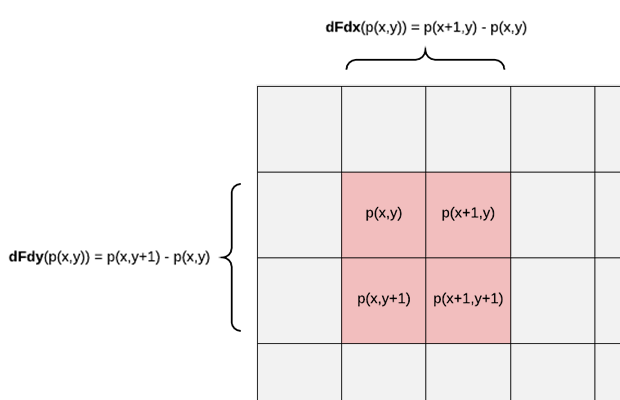
\includegraphics[width=\textwidth]{images/Shader-Derivatives.png}
\end{figure}

antialiasing,AA抗锯齿,对于一张纹理,给定UV坐标后,不仅仅是直接采样,还要考虑周围方形
区域内采样的结果,这个区域就是ddx和ddy给定的区域,在shader中调用texture时,后台进行了处理,
在一些高级的profiles中,还是允许自定义滤波窗口大小的

mipmap,在屏幕空间中,纹理坐标变换剧烈,Derivatives are used during texture sampling to
select the best mipmap level.

\subsubsection{fwidth}
GLSL中,fwidth函数返回的是X和Y方向偏导数的绝对值的和,而单方向的偏导数可以通过ddx和ddy获得

注意,这些函数与像素有关,只能在fragment/pixel shader中使用